%%%%%%%%%%%%%%%%%%%%%%%%%%%%%%%%%%%%%%%%%%%%%%%%%%%%%%%%%%%%%%%%%%%%%%%%%%%%%%%
%
% Implementation
% 
%%%%%%%%%%%%%%%%%%%%%%%%%%%%%%%%%%%%%%%%%%%%%%%%%%%%%%%%%%%%%%%%%%%%%%%%%%%%%%%


\chapter{Implementation of the task}
\label{sec:implementation}

\section{Numerical treatment of the governing equations}
The numerical results provided in this thesis study has been calculated in \textbf{FASTEST-3D} short for, \textit{Flow Analysis by Solving Transport Equation Simulating Turbulence}. The solver is developed by the LSTM branch of Friedrich Alexander University, Erlangen-Nürnberg. The FASTEST-3D solver is a finite volume solver based on co-located, block-structured meshes.The solver code is written in FORTRAN and is highly parallelizable for use in modern multi-core processors. The numerical treatment of incompressible Navier Stokes equations generated in Cartesian co-ordinates is based on the procedure proposed by \citet{peric1985finite}. It consists of a fully conservative, second-order finite volume space discretization with a collocated arrangement of variables on structural, multi-block grids. The procedure for coordinate transformation, Finite volume formulation and discretization schemes for the numerical solution of the governing equations are discussed in the following sections. These sections are summarized from the Doctoral dissertation of \citet{kumar2005modeling} and \citet{munsch2015entwicklung}.

\subsection{Coordinate transform}
The concept of coordinate transformation is to represent a complex physical domain in a much more simpler, orthogonal computational domain. The numerical treatment of a orthogonal computational domain has many advantages over non-orthogonal domains. As a consequence of coordinate transformation all the governing equations have to be represented in a general curvilinear coordinate system. The solver currently supports only orthogonal domains, this thesis study also consists of orthogonal computational domain. The coordinate transformation from Cartesian to a curvilinear orthogonal coordinate system is based on the procedure suggested by \citet{durst2008fluid}. 

Assuming the physical space in the 3-D Cartesian coordinate system is represented by $\left(x,y,z\right)$ and its corresponding domain in Curvilinear coordinate system is represented by $\left(\xi,\eta,\zeta\right)$ respectively. The relationship between the two coordinate systems are given by:

\begin{align}
 \xi &= \xi\left(x,y,z\right)\\
 \eta &= \eta\left(x,y,z\right)\\
 \zeta &= \zeta\left(x,y,z\right)
 \label{eqn:3.1}
\end{align}

\begin{figure}[h]
 \centering
 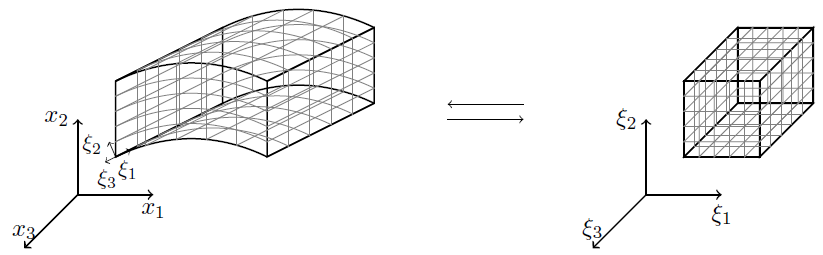
\includegraphics[height=1.8in]{coordinate_transform}
 \caption{Representation of coordinate transformation from Cartesian physical space (left) to a curvilinear orthogonal computational space (right), figure taken from \citet{munsch2015entwicklung}}
 \label{fig:3.1}
\end{figure}

The differential operators of the curvilinear coordinate domain is given by:

\begin{align}
 d\xi &= \frac{\partial{\xi}}{\partial{x}}dx+\frac{\partial{\xi}}{\partial{y}}dy+\frac{\partial{\xi}}{\partial{z}}dz\\
 d\eta &= \frac{\partial{\eta}}{\partial{x}}dx+\frac{\partial{\eta}}{\partial{y}}dy+\frac{\partial{\eta}}{\partial{z}}dz\\
 d\zeta &= \frac{\partial{\zeta}}{\partial{x}}dx+\frac{\partial{\zeta}}{\partial{y}}dy+\frac{\partial{\zeta}}{\partial{z}}dz
\end{align}

Similarly the reverse transformation from curvilinear space to the Cartesian space is denoted as follows.
\begin{align}
 x &= x\left(\xi,\eta,\zeta\right)\\
 y &= y\left(\xi,\eta,\zeta\right)\\
 z &= z\left(\xi,\eta,\zeta\right)
\end{align}

The total differential operators for reverse transformation is given by the following terms.

\begin{align}
 dx &= \frac{\partial{x}}{\partial{\xi}}d\xi+\frac{\partial{x}}{\partial{\eta}}d\eta+\frac{\partial{x}}{\partial{\zeta}}d\zeta\\
 dy &= \frac{\partial{y}}{\partial{\xi}}d\xi+\frac{\partial{y}}{\partial{\eta}}d\eta+\frac{\partial{y}}{\partial{\zeta}}d\zeta\\
 dz &= \frac{\partial{z}}{\partial{\xi}}d\xi+\frac{\partial{z}}{\partial{\eta}}d\eta+\frac{\partial{z}}{\partial{\zeta}}d\zeta
\end{align}

Both the transformations can be represented in a matrix notation as given by the following set of equations.

\begin{equation}
%\[
\begin{pmatrix}
d\xi\\
d\eta\\
d\zeta
\end{pmatrix}
=
\begin{pmatrix}
\frac{\partial{\xi}}{\partial{x}} & \frac{\partial{\xi}}{\partial{y}} & \frac{\partial{\xi}}{\partial{z}}\\
\frac{\partial{\eta}}{\partial{x}} & \frac{\partial{\eta}}{\partial{y}} & \frac{\partial{\eta}}{\partial{z}}\\
\frac{\partial{\zeta}}{\partial{x}} & \frac{\partial{\zeta}}{\partial{y}} & \frac{\partial{\zeta}}{\partial{z}}\\
\end{pmatrix}
\begin{pmatrix}
dx\\
dy\\
dz
\end{pmatrix}
%\]
\label{eqn:3.13}
\end{equation}

\begin{equation}
%\[
\begin{pmatrix}
dx\\
dy\\
dz
\end{pmatrix}
=
\begin{pmatrix}
\frac{\partial{x}}{\partial{\xi}} & \frac{\partial{x}}{\partial{\eta}} & \frac{\partial{x}}{\partial{\zeta}}\\
\frac{\partial{y}}{\partial{\xi}} & \frac{\partial{y}}{\partial{\eta}} & \frac{\partial{y}}{\partial{\zeta}}\\
\frac{\partial{z}}{\partial{\xi}} & \frac{\partial{z}}{\partial{\eta}} & \frac{\partial{z}}{\partial{\zeta}}\\
\end{pmatrix}
\begin{pmatrix}
d\xi\\
d\eta\\
d\zeta
\end{pmatrix}
%\]
\label{eqn:3.14}
\end{equation}

The matrices in the equations \ref{eqn:3.13} and \ref{eqn:3.14} are termed as transformation or \textit{Jacobian} matrices. The matrices are referenced as $a_{ij}$ and $b_{ij}$ respectively for easier notation. In general applications the computational grid is generated in the physical space. The relations in mapping to the curvilinear space as given by the set of equations \ref{eqn:3.1} are unknown and consequently the transformation matrix $a_{ij}$ as represented in the equation \ref{eqn:3.13} is also unknown. 

The transformation matrix $a_{ij}$ can be calculated from the following relationship:

\begin{equation}
\begin{pmatrix}
\frac{\partial{\xi}}{\partial{x}} & \frac{\partial{\xi}}{\partial{y}} & \frac{\partial{\xi}}{\partial{z}}\\
\frac{\partial{\eta}}{\partial{x}} & \frac{\partial{\eta}}{\partial{y}} & \frac{\partial{\eta}}{\partial{z}}\\
\frac{\partial{\zeta}}{\partial{x}} & \frac{\partial{\zeta}}{\partial{y}} & \frac{\partial{\zeta}}{\partial{z}}\\
\end{pmatrix} 
=
\begin{pmatrix}
\frac{\partial{x}}{\partial{\xi}} & \frac{\partial{x}}{\partial{\eta}} & \frac{\partial{x}}{\partial{\zeta}}\\
\frac{\partial{y}}{\partial{\xi}} & \frac{\partial{y}}{\partial{\eta}} & \frac{\partial{y}}{\partial{\zeta}}\\
\frac{\partial{z}}{\partial{\xi}} & \frac{\partial{z}}{\partial{\eta}} & \frac{\partial{z}}{\partial{\zeta}}
\end{pmatrix}^{-1}
\label{eqn:3.15}
\end{equation}
This can also be represented using referenced notation as 
\begin{equation}
\left(a_{ij}\right) = \left(b_{ij}\right)^{-1}
\label{eqn:3.16}
\end{equation}

The inverse of the transformation matrix $b_{ij}$ is calculated as represented below in the equation \ref{eqn:3.17}.
\begin{equation}
\left(a_{ij}\right) = \left(b_{ij}\right)^{-1} = \frac{adj\left(b_{ij}\right)}{\det\left(b_{ij}\right)} 
\label{eqn:3.17}
\end{equation}	
where, $adj\left(b_{ij}\right)$ is the transpose of the cofactor matrix of $\left(b_{ij}\right)$ and the determinant of the transformation matrix is the \textit{Jacobian} and is denoted by J. Thus, the inverse of the transformation matrix can be rewritten as 
\begin{equation}
\left(b_{ij}\right)^{-1} = \frac{1}{J}
\begin{pmatrix}
\beta_{11} & \beta_{12} & \beta_{13}\\
\beta_{21} & \beta_{22} & \beta_{23}\\
\beta_{31} & \beta_{32} & \beta_{33}
\end{pmatrix}
\label{eqn:3.18}
\end{equation}
where the coefficients are calculated as 
\begin{align}
\beta_{11} &= \frac{\partial{y}}{\partial{\eta}}\frac{\partial{z}}{\partial{\zeta}} - \frac{\partial{y}}{\partial{\zeta}}\frac{\partial{z}}{\partial{\eta}} = \frac{\partial{\xi}}{\partial{x}}J\\
	\beta_{12} &= \frac{\partial{x}}{\partial{\zeta}}\frac{\partial{z}}{\partial{\eta}} - \frac{\partial{x}}{\partial{\eta}}\frac{\partial{z}}{\partial{\zeta}} = \frac{\partial{\xi}}{\partial{y}}J\\
	\beta_{13} &= \frac{\partial{x}}{\partial{\eta}}\frac{\partial{y}}{\partial{\zeta}} - \frac{\partial{x}}{\partial{\zeta}}\frac{\partial{y}}{\partial{\eta}} = \frac{\partial{\xi}}{\partial{z}}J\\
	\beta_{21} &= \frac{\partial{y}}{\partial{\zeta}}\frac{\partial{z}}{\partial{\xi}} - \frac{\partial{y}}{\partial{\xi}}\frac{\partial{z}}{\partial{\zeta}} = \frac{\partial{\eta}}{\partial{x}}J\\
	\beta_{22} &= \frac{\partial{x}}{\partial{\xi}}\frac{\partial{z}}{\partial{\zeta}} - \frac{\partial{x}}{\partial{\zeta}}\frac{\partial{z}}{\partial{\xi}} = \frac{\partial{\eta}}{\partial{y}}J\\
	\beta_{23} &= \frac{\partial{x}}{\partial{\zeta}}\frac{\partial{y}}{\partial{\xi}} - \frac{\partial{x}}{\partial{\xi}}\frac{\partial{y}}{\partial{\zeta}} = \frac{\partial{\eta}}{\partial{z}}J\\
	\beta_{31} &= \frac{\partial{y}}{\partial{\xi}}\frac{\partial{z}}{\partial{\eta}} - \frac{\partial{y}}{\partial{\eta}}\frac{\partial{z}}{\partial{\xi}} = \frac{\partial{\zeta}}{\partial{x}}J\\
	\beta_{32} &= \frac{\partial{x}}{\partial{\eta}}\frac{\partial{z}}{\partial{\xi}} - \frac{\partial{x}}{\partial{\xi}}\frac{\partial{z}}{\partial{\eta}} = \frac{\partial{\zeta}}{\partial{y}}J\\
	\beta_{33} &= \frac{\partial{x}}{\partial{\eta}}\frac{\partial{y}}{\partial{\eta}} - \frac{\partial{x}}{\partial{\eta}}\frac{\partial{y}}{\partial{\xi}} = \frac{\partial{\zeta}}{\partial{z}}J
 \label{eqn:3.19}
\end{align}

The gradients of a scalar quantity along the Cartesian coordinates are transformed via the chain rule to the curvilinear coordinate system:

\begin{equation}
 \frac{\partial\phi}{\partial{x_{i}}} = \frac{\partial\phi}{\partial{\xi_j}}\frac{\partial{\xi_j}}{\partial{x_i}} = \frac{\partial\phi}{\partial{\xi_j}}\frac{\beta_{ij}}{J}
 \label{eqn:3.28}
\end{equation}

The divergence of a vector quantity $\phi_{i}$ can be calculated as follows:
\begin{equation}
\frac{\partial{\phi_i}}{\partial{x}} = \frac{\partial{\phi_{i}}}{\partial{\xi_{j}}}\frac{\beta_{ij}}{J}
\label{eqn:3.29}
\end{equation}

The Laplacian of a scalar quantity is represented in the computational space as defined below.

\begin{equation}
\frac{\partial}{\partial{x_i}}\left(\frac{\partial\phi}{\partial{x_i}}\right) = \frac{\partial}{\partial{\xi_j}}\left(\frac{\partial\phi}{\partial{\xi_k}}\frac{\beta_{ki}}{J}\frac{\beta_{ji}}{J}\right)
\label{eqn:3.30}
\end{equation}

In a Cartesian coordinate or physical space, the general transport equation for an \textit{incompressible Newtonian fluid} with a transport variable $\Phi$ is represented as,
\begin{equation}
\frac{\partial{\left(\rho\Phi\right)}}{\partial{t}}+\frac{\partial{\left({\rho}{u_i}\Phi\right)}}{\partial{x_i}} = \frac{\partial}{\partial{x_i}}\left(\Gamma_{\Phi}\frac{\partial{\Phi}}{\partial{x_i}}\right)+S_{\Phi}
\label{eqn:3.31}
\end{equation}
where the source term $S_{\Phi}$ is represented as follows.
\begin{equation}
S_{\Phi} = -\frac{\partial{p}}{\partial{x_i}}+{\rho}gi
\end{equation}

In the equation \ref{eqn:3.31}, the term $\Gamma_{\Phi}$ represents the diffusion coefficient of the transport equation. The transformed equation in curvilinear or computational space is represented based on the gradient, divergence and Laplacian as represented in the equations \ref{eqn:3.28}, \ref{eqn:3.29} and \ref{eqn:3.30} respectively. 
\begin{equation}
\frac{\partial{\left(\rho\Phi\right)}}{\partial{t}}+\frac{1}{J}\frac{\partial{\left({\rho}{U_j}{\Phi}J\right)}}{\partial{\xi_j}} = \frac{1}{J}\frac{\partial}{\partial{\xi_j}}\left(\frac{\Gamma_{\Phi}}{J}\frac{\partial{\Phi}}{\partial{\xi_k}}B_{kj}\right)+S_{\Phi}
\label{eqn3.33}
\end{equation}

The transformed source term in curvilinear coordinate system is represented as,
\begin{equation}
S_{\Phi} = -\frac{1}{J}\left(\frac{\partial{p}}{\partial{\xi_k}}\beta_{ki}\right)+{\rho}gi
\end{equation}

The velocity component $U_j=\left(U,V,W\right)$ describes the \textit{contravariant velocity} components which are based on the metric coefficients $\beta_{ij}$, the Jacobian J and the respective Cartesian velocity components. They can be evaluated as follows.
\begin{equation}
U_j = \frac{1}{J}\left(u{\beta_{j1}}+v{\beta_{j2}}+w{\beta_{j3}}\right)=\frac{1}{J}\left(u_{n}{\beta_{jn}}\right)
\end{equation}

The coefficients $B_{kj}$ are described as:
\begin{equation}
B_{kj} = \beta_{km}\beta_{jm} = \beta_{k1}\beta_{j1}+\beta_{k2}\beta_{j2}+\beta_{k3}\beta_{j3}
\label{eqn:3.36}
\end{equation}

If the grid is orthogonal in the physical space, the off-diagonal elements $\beta_{ij}$ in the transformation tensor vanishes and the general equation will be similar to the Cartesian form. The elements $b_{ij}$ can be approximated at the control volume (CV) centers using second order central difference scheme.
\begin{equation}
\left(b_{ij}\right)_P = \left(\frac{\partial x_i}{\partial \xi}\right)_P \approx \frac{x_{i,e} - x_{i,w}}{\delta \xi}
\label{eqn:3.37}
\end{equation}
The distance between the centers of the control volumes is assumed to be 1, i.e. $\delta \xi = 1$. The $j^{th}$ column elements of $b_{ij}$ for the control volume represented in figure \ref{fig:3.2} can be represented as follows:
\begin{figure}[h]
\centering
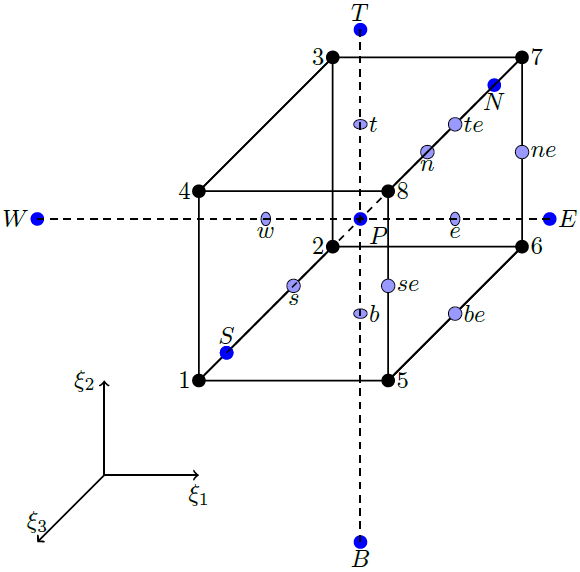
\includegraphics[height=3.5in]{cv}
\caption{Representational control volume in the computational domain, picture taken from \citet{munsch2015entwicklung}}
\label{fig:3.2}
\end{figure}

\begin{align}
	\left(b_{i1}\right)_P &= \left(\frac{\partial x_i}{\partial \xi}\right)_P \approx \frac{x_{i,5} + x_{i,6} + x_{i,7} + x_{i,8}}{4} - \frac{x_{i,1} + x_{i,2} + x_{i,3} + x_{i,4}}{4}\\
	\left(b_{i2}\right)_P &= \left(\frac{\partial x_i}{\partial \eta}\right)_P \approx \frac{x_{i,3} + x_{i,4} + x_{i,7} + x_{i,8}}{4} - \frac{x_{i,1} + x_{i,2} + x_{i,5} + x_{i,6}}{4}\\
	\left(b_{i3}\right)_P &= \left(\frac{\partial x_i}{\partial \zeta}\right)_P \approx \frac{x_{i,1} + x_{i,4} + x_{i,5} + x_{i,8}}{4} - \frac{x_{i,2} + x_{i,3} + x_{i,6} + x_{i,7}}{4}
	\label{eqn:3.40}
\end{align}

The numerical treatment of the governing equation is done by Finite volume method. The discretization of the equation is presented in the following section.

\section{Finite Volume method to solve the Navier Stokes equation}

The transformed transport equation in the conservative form is represented in the following equation. 
\begin{equation}
\int_{V_{\xi}} \frac{\partial \Phi}{\partial t}J dV_{\xi} + \int_{V_{\xi}} \frac{\partial \left(U_j \Phi\right)}{\partial \xi_j} dV_{\xi} = \int_{V_{\xi}} \frac{1}{J} \left(\Gamma_{\Phi} \frac{\partial \Phi}{\partial \xi_k} B_{kj} \right) dV_{\xi} + \int_{V_{\xi}} JS_{\Phi} dV_{\xi}
\label{eqn:3.41}
\end{equation}

The control volume $\left(CV\right)$ in the computational domain is related to a CV in physical domain as given below.
\begin{align}
dV_{\xi} &= d \xi d \eta d \zeta = 1\\
dV &= dx dy dz = J d \xi d \eta d \zeta = J
\label{eqn:3.43}
\end{align}

Applying the \textit{Gauss divergence} to the equation \ref{eqn:3.41}, the volume integral of the fluxes are transformed to the surface integral and the equation is rewritten as: 

\begin{equation}
\int_{V_{\xi}} \frac{\partial \Phi}{\partial t}J dV_{\xi} + \int_{A_{\xi}} U_j \Phi dA_{{\xi}_j} = \int_{A_{\xi}} \frac{1}{J} \left(\Gamma_{\Phi} \frac{\partial \Phi}{\partial \xi_k} B_{kj} \right) dA_{{\xi}_j} + \int_{V_{\xi}} JS_{\Phi} dV_{\xi}
\label{eqn:3.44}
\end{equation}

where, $A_{{\xi}_j}$ is the area vectors of the control volume surfaces. 


